\section{Results}

\subsection{Experiment 1}

We use the
\href{https://statistics.laerd.com/statistical-guides/pearson-correlation-coefficient-statistical-guide.php}{Pearson
correlation coefficient} to determine the similarity between the
derivatives of the global Q function critic and the local approximations
we use a-la DDPG.

We wish to approximate this global Q using less expensive local Q approximator functions. We can ignore the magnitude and actual values of the two functions as we only wish to examine the updates, i.e.~derivatives of these functions. Thus,
we attempt to \textbf{find a positive correlation between
\(\frac{\partial Q_{global}}{\partial t}\) and
\(\frac{\partial Q_{local}}{\partial t}\).}

This table can be used to roughly understand
the importance of correlations between two functions.

\begin{figure}[h]
\centering
\begin{subfigure}{.5\textwidth}
  \centering
  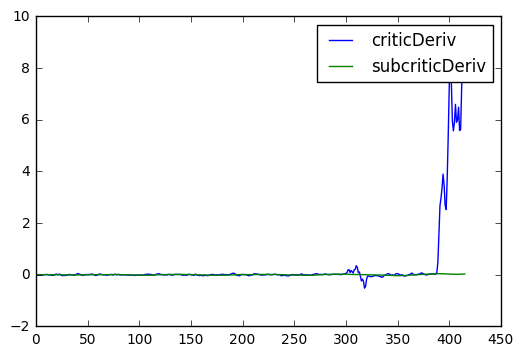
\includegraphics[width=.6\linewidth]{exp1_analysis_1_1.png}
  \caption{Critic and subcritic derivatives}
  \label{fig:sub1}
\end{subfigure}%
\begin{subfigure}{.5\textwidth}
  \centering
  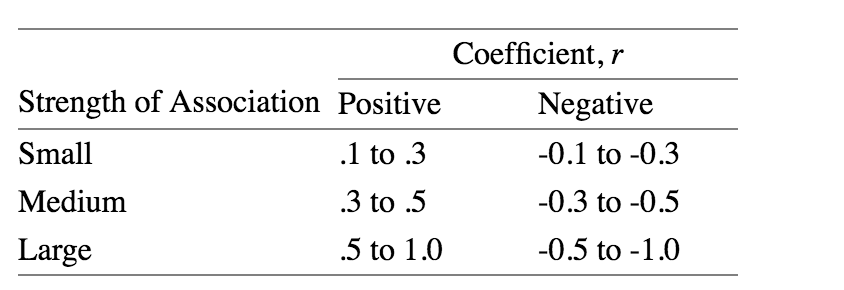
\includegraphics[width=.6\linewidth]{pearson_table.png}
  \caption{Pearson interpretation}
  \label{fig:sub2}
\end{subfigure}
\caption{Analysis figures}
\label{fig:test}
\end{figure}

In the mountain car experiment, we find a Pearson r-value of
0.389. Thus, we can infer that there is a medium association between the derivatives of the global and local function.

\subsection{Experiment 2}
The second experiment implemented the local training paradigm suggested above. We tested our results with a simple 1D synthetic environment where the agent was given 100 reward for stepping on a block 100 steps to the right, a -1 reward for moving left and 0 reward for all positions between the starting block and the 100 reward block.

The agent easily learned this environment using a two layer network. To generalize our results, we moved onto a more difficult environment, Mountain Car. This environment requires an agent to drive a car up a mountain. 

However, the car doesn't have enough power to make it up the mountain and must first drive back, the direction opposite the goal, then drive forward to successfully complete the environment. 

We successfully solved the environment with small simple networks, however, if we tried to use multiple layers the local Q functions began to diverge. We believe this is a result of the high variance in the local environments of each neuron as a result of constantly feeding in values and will require more evaluation to correct this issue.